\section{Technologies}
Voici un lien vers la vid\'eo YouTube :  
\href{https://youtu.be/xMGjdUp73b8?list=PLSiaem2m0wQ0eRmm17OQ-GjAeBgjRirO2}{Cliquez ici pour voir la vid\'eo}

\begin{figure}[H] % H force l'affichage ici
    \centering
    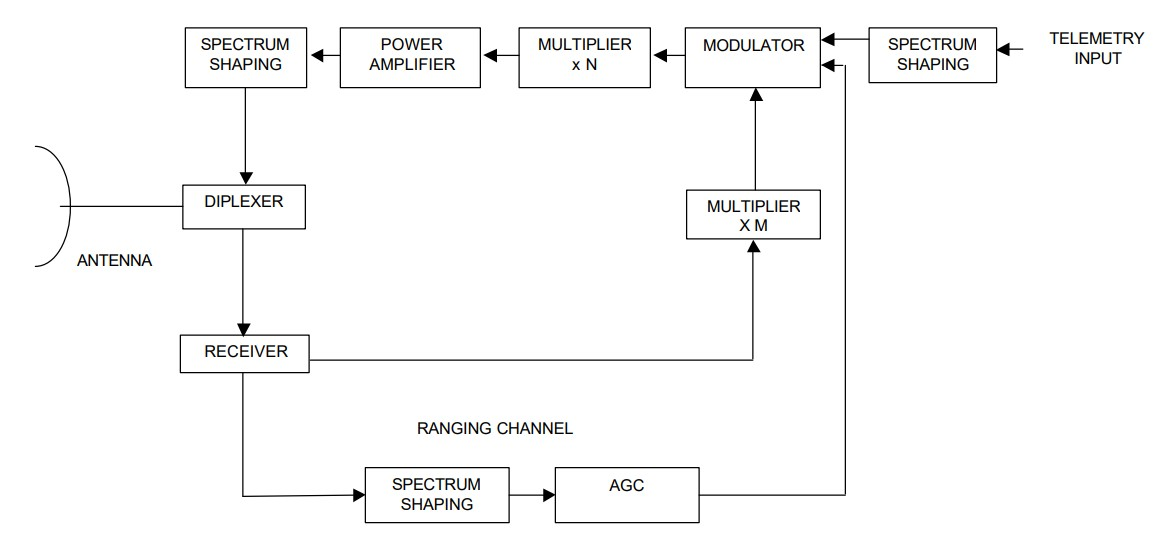
\includegraphics[width=0.8\textwidth]{figures/6-65.jpg}
    \caption{\href{https://www.researchgate.net/publication/242211974_CCSDS_-_SFCG_EFFICIENT_MODULATION_METHODS_STUDY_A_COMPARISON_OF_MODULATION_SCHEMES_PHASE_2_SPECTRUM_SHAPING}{Simplified Block Diagram of Spacecraft Radio Frequency Subsystem.}}
    \label{fig:communication2}
\end{figure}

\begin{itemize}
    \item Le mat\'eriel et les logiciels de communication diff\`erent entre le vaisseau spatial et le sol en raison des contraintes d’espace et d’alimentation disponibles.
    \item Typiquement :
    \begin{itemize}
        \item L’antenne au sol est plus grande que celle du vaisseau spatial afin d’augmenter le gain ainsi que le bilan de liaison.
        \item Les contraintes de masse sont moins restrictives au sol.
        \item Les antennes terrestres transmettent \'egalement avec une puissance beaucoup plus \'elev\'ee, augmentant ainsi le gain avec moins de contraintes de puissance.
    \end{itemize}
    \item Nous nous concentrerons sur la technologie embarqu\'ee des vaisseaux spatiaux, notamment :
    \begin{itemize}
        \item Les antennes
        \item Les \'emetteurs-r\'ecepteurs
        \item Les filtres
        \item Les duplexeurs
    \end{itemize}
\end{itemize}

\begin{figure}[H]
    \centering
    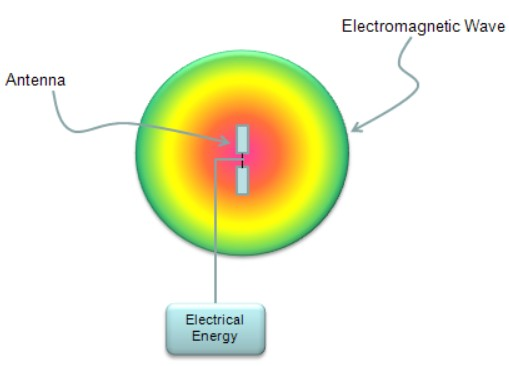
\includegraphics[width=0.8\textwidth]{figures/6-66.jpg}
    \caption{Antenna concept. Image by Share Tech Note.}
    \label{fig:communication3}
\end{figure}

\begin{itemize}
    \item Les antennes sont des circuits (fils, ouvertures) qui interagissent avec les ondes \'electromagn\'etiques en transformant les champs \'electriques en courants (et vice-versa).
    \item Elles re\c{c}oivent et transmettent l’\'energie RF (radiofr\'equence).
    \item La taille et le type d’antenne s\'electionn\'es sont directement li\'es \`a la fr\'equence et au gain requis.
\end{itemize}

\begin{figure}[H]
    \centering
    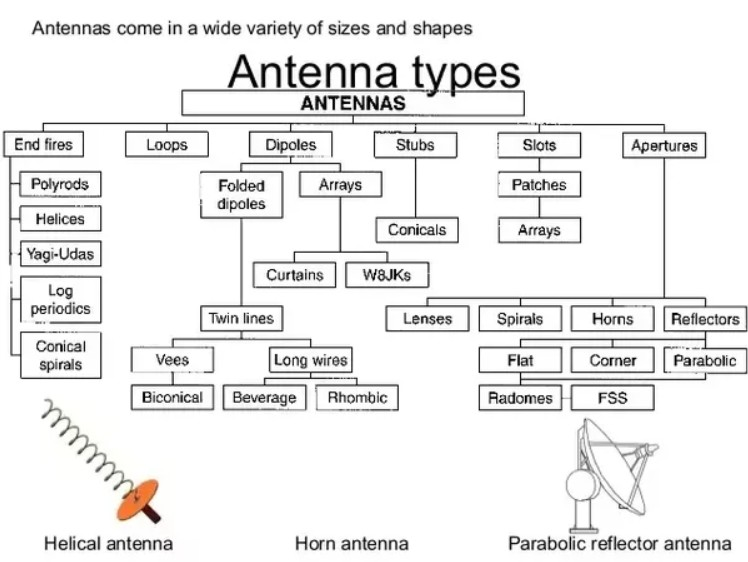
\includegraphics[width=0.8\textwidth]{figures/6-67.jpg}
    \caption{\href{https://www.slideserve.com/tariq/antennas-powerpoint-ppt-presentation}{Various sizes and shapes of antennas. Image by QPH.}}
    \label{fig:communication4}
\end{figure}

\textbf{There are different types of antennas:}

\begin{figure}[H]
    \centering
    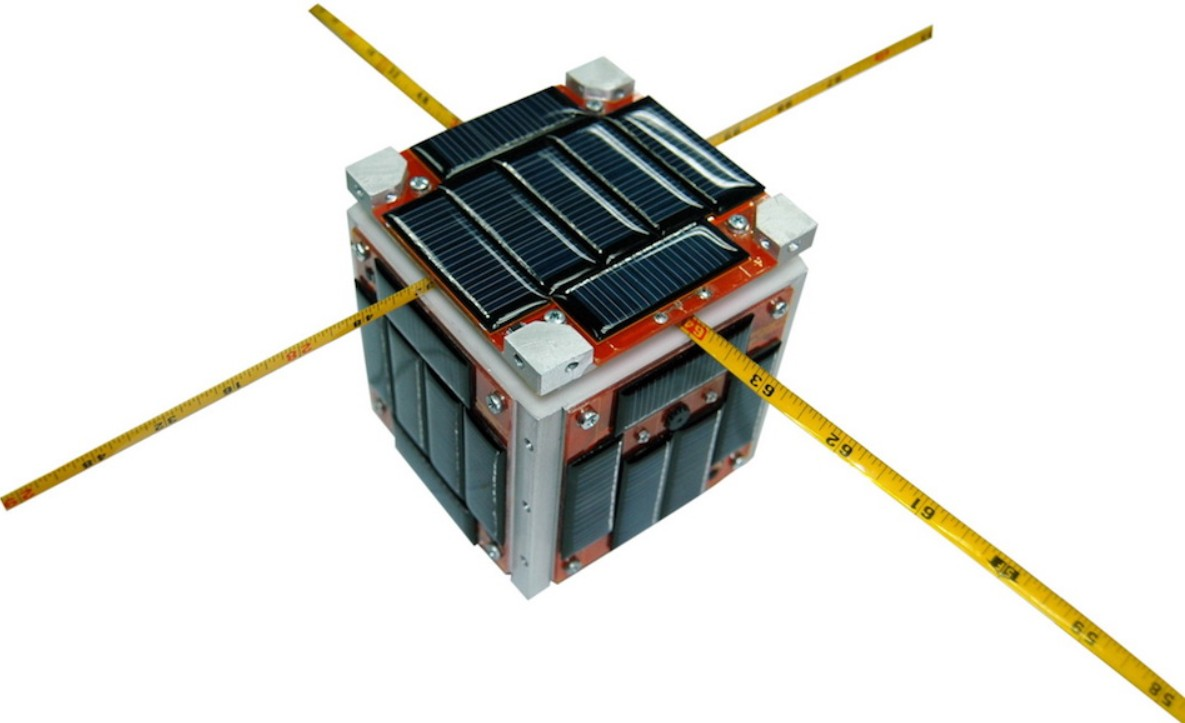
\includegraphics[width=0.8\textwidth]{figures/6-68.jpg}
    \caption{\href{https://phys.org/news/2022-09-team-amateurs-built-satellite-nasa.html}{A CubeSat with antennae made of measuring tape. Image by Net DNA.}}
    \label{fig:communication5}
\end{figure}

\begin{figure}[H]
    \centering
    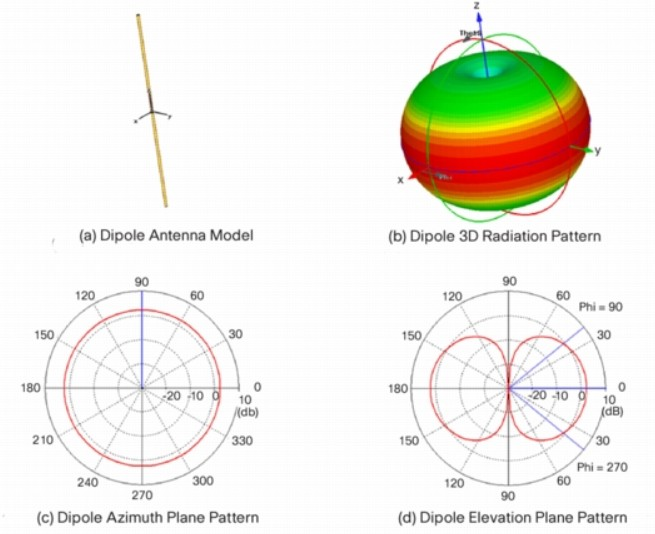
\includegraphics[width=0.8\textwidth]{figures/6-69.jpg}
    \caption{Dipole Antenna 3D Radiation Pattern. Image by Raymaps.}
    \label{fig:communication6}
\end{figure}

\begin{itemize}
    \item Une antenne omnidirectionnelle rayonne isotropiquement dans toutes les directions, de sorte que la densit\'e de puissance \'emise \`a une distance \( R \gg \lambda \) est donn\'ee par :
    \[ P\left(\frac{W}{m^2}\right) = \frac{P_T}{4\pi R^2} \]
    \item La plupart des antennes sont directionnelles, c'est-\`a-dire que l'intensit\'e de la puissance rayonn\'ee d\'epend de la direction.
    \item Les diagrammes de gain illustrent la directivit\'e de l'antenne.
    \item La directivit\'e d'une antenne permet d'obtenir un gain plus \'elev\'e dans une direction sp\'ecifique, mais le satellite doit orienter cet axe vers la station au sol avec plus de pr\'ecision pour b\'en\'eficier de ce gain am\'elior\'e, ce qui repr\'esente un compromis en termes de complexit\'e du syst\`eme ADCS.
\end{itemize}

\begin{figure}[H]
    \centering
    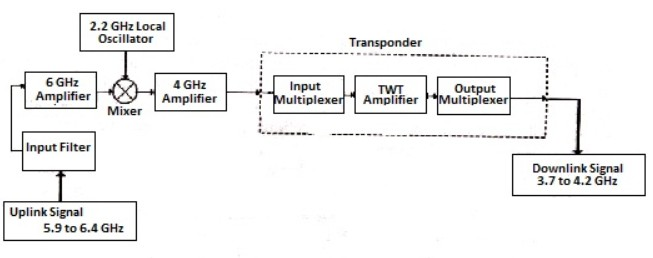
\includegraphics[width=0.8\textwidth]{figures/6-80.jpg}
    \caption{A satellite communication system is mentioned, where the role of a transponder is clearly magnified. Image by Daenotes.}
    \label{fig:communication7}
\end{figure}

\begin{itemize}
    \item Un transpondeur de satellite de communication est un ensemble d'unit\'es interconnect\'ees formant un canal de communication entre les antennes de r\'eception et d’\'emission.
    \item Il est principalement utilis\'e pour transf\'erer les signaux re\c{c}us.
    \item Un transpondeur est typiquement compos\'e de :
    \begin{itemize}
        \item Un dispositif de limitation de bande en entr\'ee (\textbf{filtre passe-bande en entr\'ee}),
        \item Un amplificateur \`a faible bruit (\textbf{LNA - Low Noise Amplifier}) pour amplifier les signaux faibles re\c{c}us de la station terrestre,
        \item Un traducteur de fr\'equence (\textbf{oscillateur et m\'elangeur de fr\'equence}) pour convertir la fr\'equence du signal re\c{c}u \`a celle requise pour l'\'emission,
        \item Un \textbf{filtre passe-bande en sortie},
        \item Un \textbf{amplificateur de puissance} (tube \`a ondes progressives ou amplificateur \`a semi-conducteurs).
    \end{itemize}
\end{itemize}
